\begin{frame}{Miscellaneous}
\begin{enumerate}
\conti
\item The lengths of two parallel chords of a circle are 6 cm and 8 cm. If the smaller chord is
at distance 4 cm from the centre, what is the
distance of the other chord from the centre?
\seti
\end{enumerate}
\textbf{Solution:} 
\begin{figure}[!ht]
\resizebox{0.45\linewidth}{!}
{
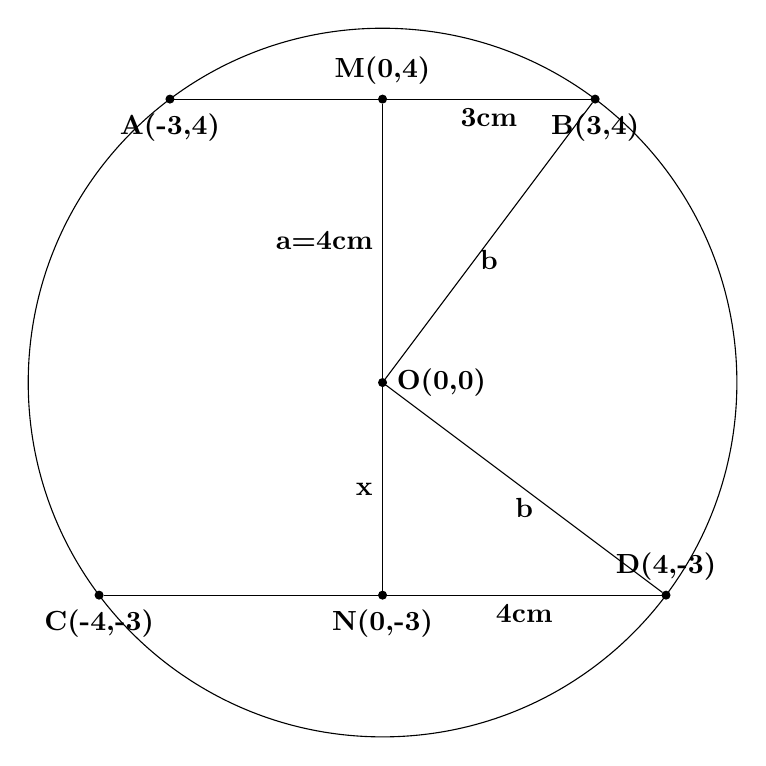
\begin{tikzpicture}[scale =0.9,>=stealth,point/.style = {draw, circle, fill = black, inner sep = 1pt},]
\draw (0,0)circle (5cm);
\node (O) at (0,0)[point,label=right :$\textbf{O(0,0)}$] {};
\node (A) at (-3,4)[point,label=below :$\textbf{A(-3,4)}$] {};
\node (B) at (3,4)[point,label=below :$\textbf{B(3,4)}$] {};
\node (C) at (-4,-3)[point,label=below :$\textbf{C(-4,-3)}$] {};
\node (D) at (4,-3)[point,label=above :$\textbf{D(4,-3)}$] {};
\node (M) at (0,4)[point,label=above :$\textbf{M(0,4)}$] {};
\node (N) at (0,-3)[point,label=below :$\textbf{N(0,-3)}$] {};
\draw (A)--(B);
\draw (C)--(D);
\draw (O)--node[left] {$\textbf{a=4cm}$}(M);
\draw (O)--node[left] {$\textbf{x}$}(N);
\draw (O)--node[below] {$\textbf{b}$}(B);
\draw (O)--node[below] {$\textbf{b}$}(D);
\draw (M)--node[below] {$\textbf{3cm}$}(B);
\draw (N)--node[below] {$\textbf{4cm}$}(D);
\end{tikzpicture}

}
\caption{tikz figure}
\label{fig:foo}
\end{figure}
\end{frame}
\begin{frame}
\begin{figure}[!ht]
\resizebox{0.45\linewidth}{!}
{
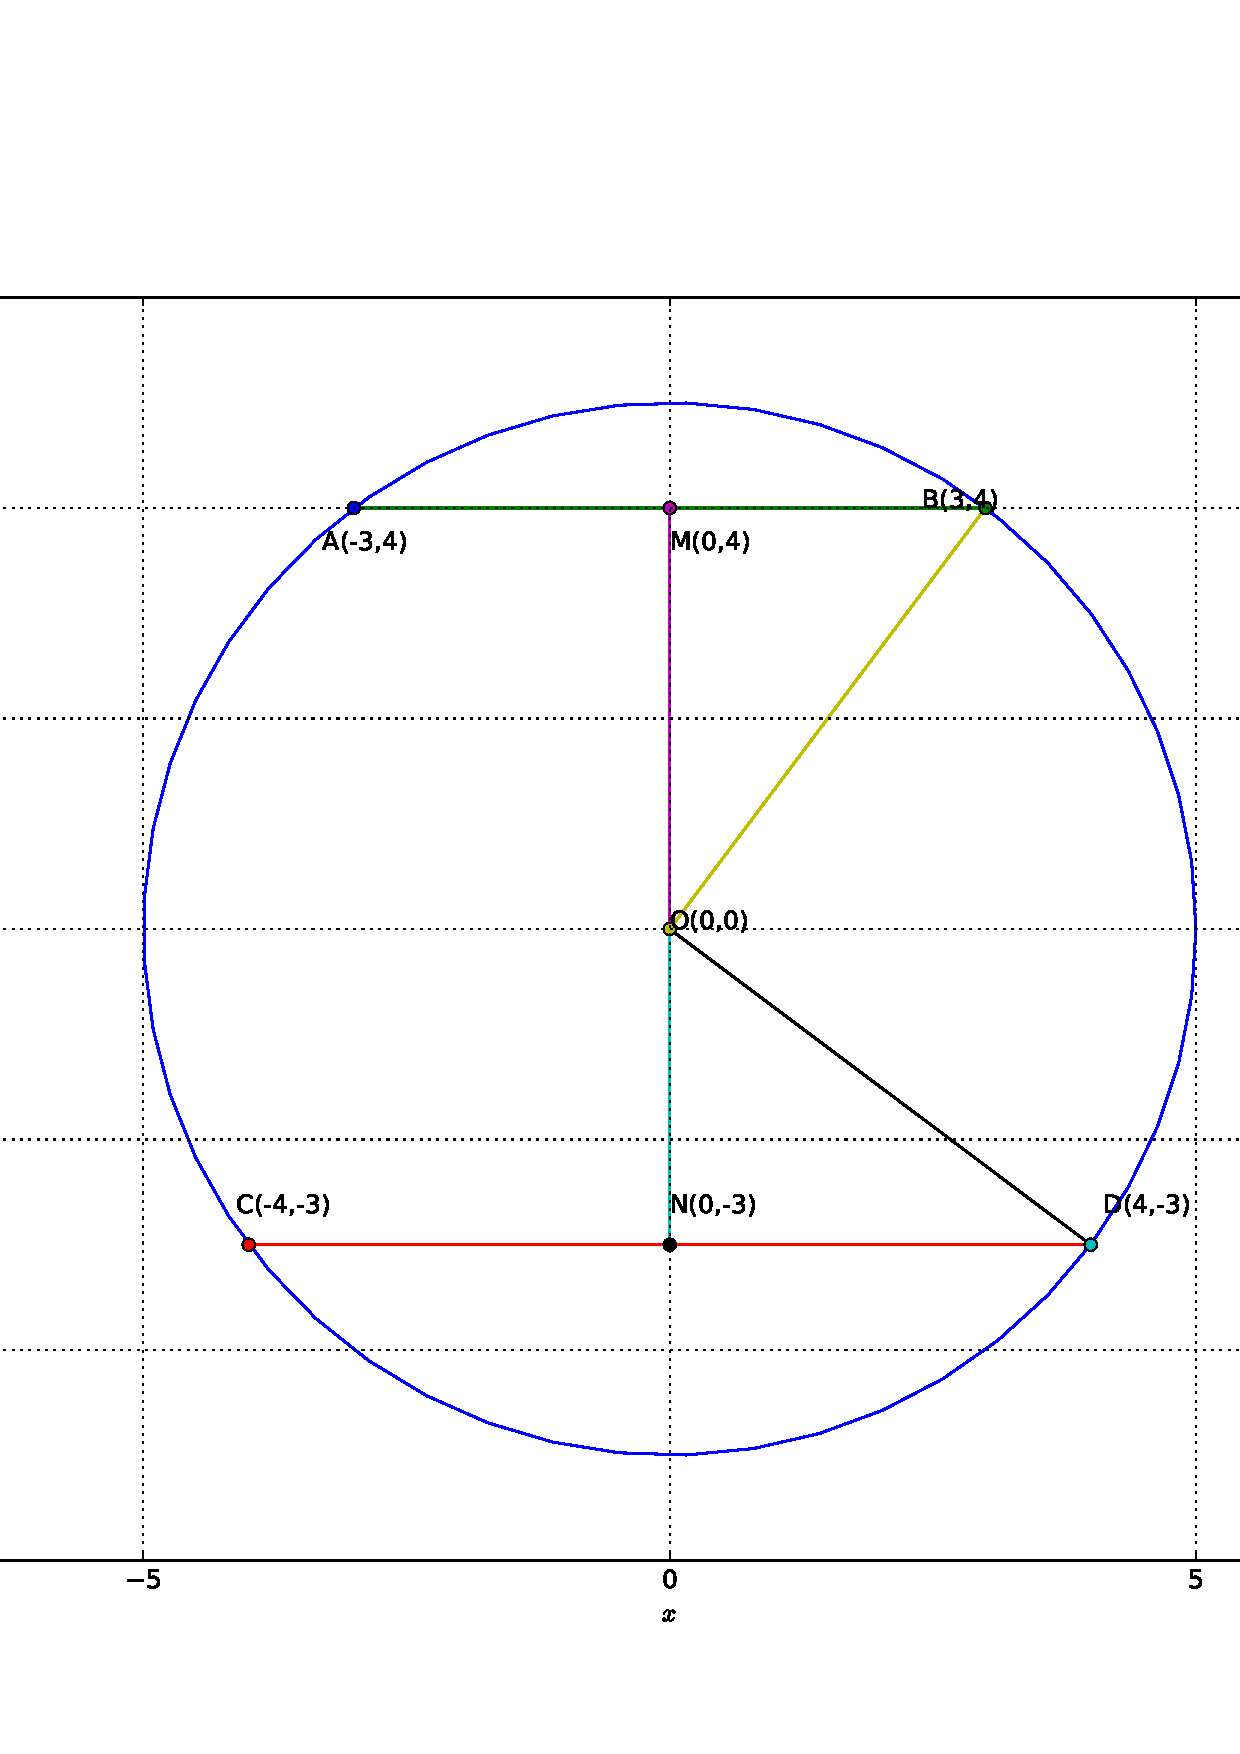
\includegraphics[scale=1.2]{./figs/misc.png}
}
\caption{Python generated figure}
\label{fig:foo}
\end{figure}
Apply Baudhayana theorem for $\triangle{MOB}$ and $\triangle{NOD}$
\begin{align*}
a^2+(3)^2=(b)^2 \\
x^2+(4)^2=b^2
\end{align*}
\begin{itemize}
\item \textbf{python:} \url{https://github.com/d-DP/geometryy/blob/master/codes/misc.py}
\item \textbf{tikz:} \url{https://github.com/d-DP/geometryy/blob/master/figs/misc.tex}
\end{itemize}
\end{frame}